\documentclass[a4paper, 10pt, ]{article}

\input{./COMMONFILES/preamble.tex}

% -----------------------------------------------------------------------------

\def\oznacenieCelku{Kolekcia učebných textov}

% -----------------------------------------------------------------------------


\def\KUTporadoveCislo{devMOTOR\_part1}

% \def\oznacenieVerzie{v0.9}
\def\oznacenieVerzie{\phantom{v1.0}}

\def\mesiacRok{august 2025}

\def\authorslabel{AS}






% -----------------------------------------------------------------------------

\begin{document}

% -----------------------------------------------------------------------------
% Uvodny nadpis

\noindent
\parbox[t][18mm][c]{0.3\textwidth}{%
\raisebox{-0.9\height}{%
\phantom{.}\includegraphics[height=18mm]{./COMMONFILES/URKFEIlogo.pdf}%
}%
}%
\parbox[t][18mm][c]{0.7\textwidth}{%
\raggedleft

\sffamily
\fontsize{16pt}{18pt}
\fontseries{sbc}
\selectfont

\noindent
\textcolor[rgb]{0.75, 0.75, 0.75}{\textls[25]{\oznacenieCelku}}
}%

\noindent
\parbox[t][16mm][b]{0.5\textwidth}{%
\raggedright

\color{Gray}
\sffamily

\fontsize{12pt}{12pt}
\selectfont
\mesiacRok

\fontsize{6pt}{10pt}
\selectfont
github.com/OkoliePracovnehoBodu/KUT

\fontsize{8pt}{10pt}
\selectfont
\authorslabel




}%
\parbox[t][16mm][b]{0.5\textwidth}{%
\raggedleft

\sffamily

\fontsize{6pt}{6pt}
\selectfont

\textcolor[rgb]{0.68, 0.68, 0.68}{\oznacenieVerzie}


\fontsize{14pt}{14pt}
\selectfont

\bfseries

\includegraphics[height=12pt]{./COMMONFILES/KUT_logo_v0.1.pdf}%
{%
\textls[-50]{\KUTporadoveCislo}
}%
}%

% -----------------------------------------------------------------------------




\vspace{6mm}

% ---------------------------------------------
\sffamily
\bfseries
\fontsize{18pt}{21pt}
\selectfont

\begin{flushleft}
    Laboratórne zariadenie mot\_UNO\_mk2:\\ Orientačný prehľad
\end{flushleft}

\bigskip

% -----------------------------------------------------------------------------
\normalsize
\normalfont
% -----------------------------------------------------------------------------

\lstset{style=mystyle}










\noindent
\lettrine[lines=1, nindent=1pt, loversize=0.0]{C}{ieľom} 
textu je opis laboratórneho zariadenia mot\_UNO\_mk2 predstavujúceho fyzický model spojitého dynamického systému.







\section{Opis dynamického systému}

Táto dynamická model obsahuje napájací zdroj z notebooku, menič napätia a prúdu, potenciometer (ako vstupný signál), Arduino Uno a samotný motor.
Motor ako vstupný signál prijíma napätie v rozsahu 0 – 12 [V], čo zodpovedá 0 – 255 diskrétnym jednotkám. Jeho výstup sa meria s rozlíšením 10 bitov, teda v rozsahu od 0 do 1023 diskrétnych jednotiek.





\section{Rozsahy a jednotky signálov}






\section{Schematické znázornenie}

\begin{center}

    \vbox{%


        \makebox[\textwidth][c]{%
        \includegraphics[width=1\textwidth,keepaspectratio]{motor_scheme.png}
        }

        \figcaption{ 
            Fotografia.
        }
        \label{motor_scheme}
    }%vbox

\end{center}








\section{Foto dokumnetácia}









\begin{center}

    \vbox{%
        \makebox[\textwidth][c]{%
        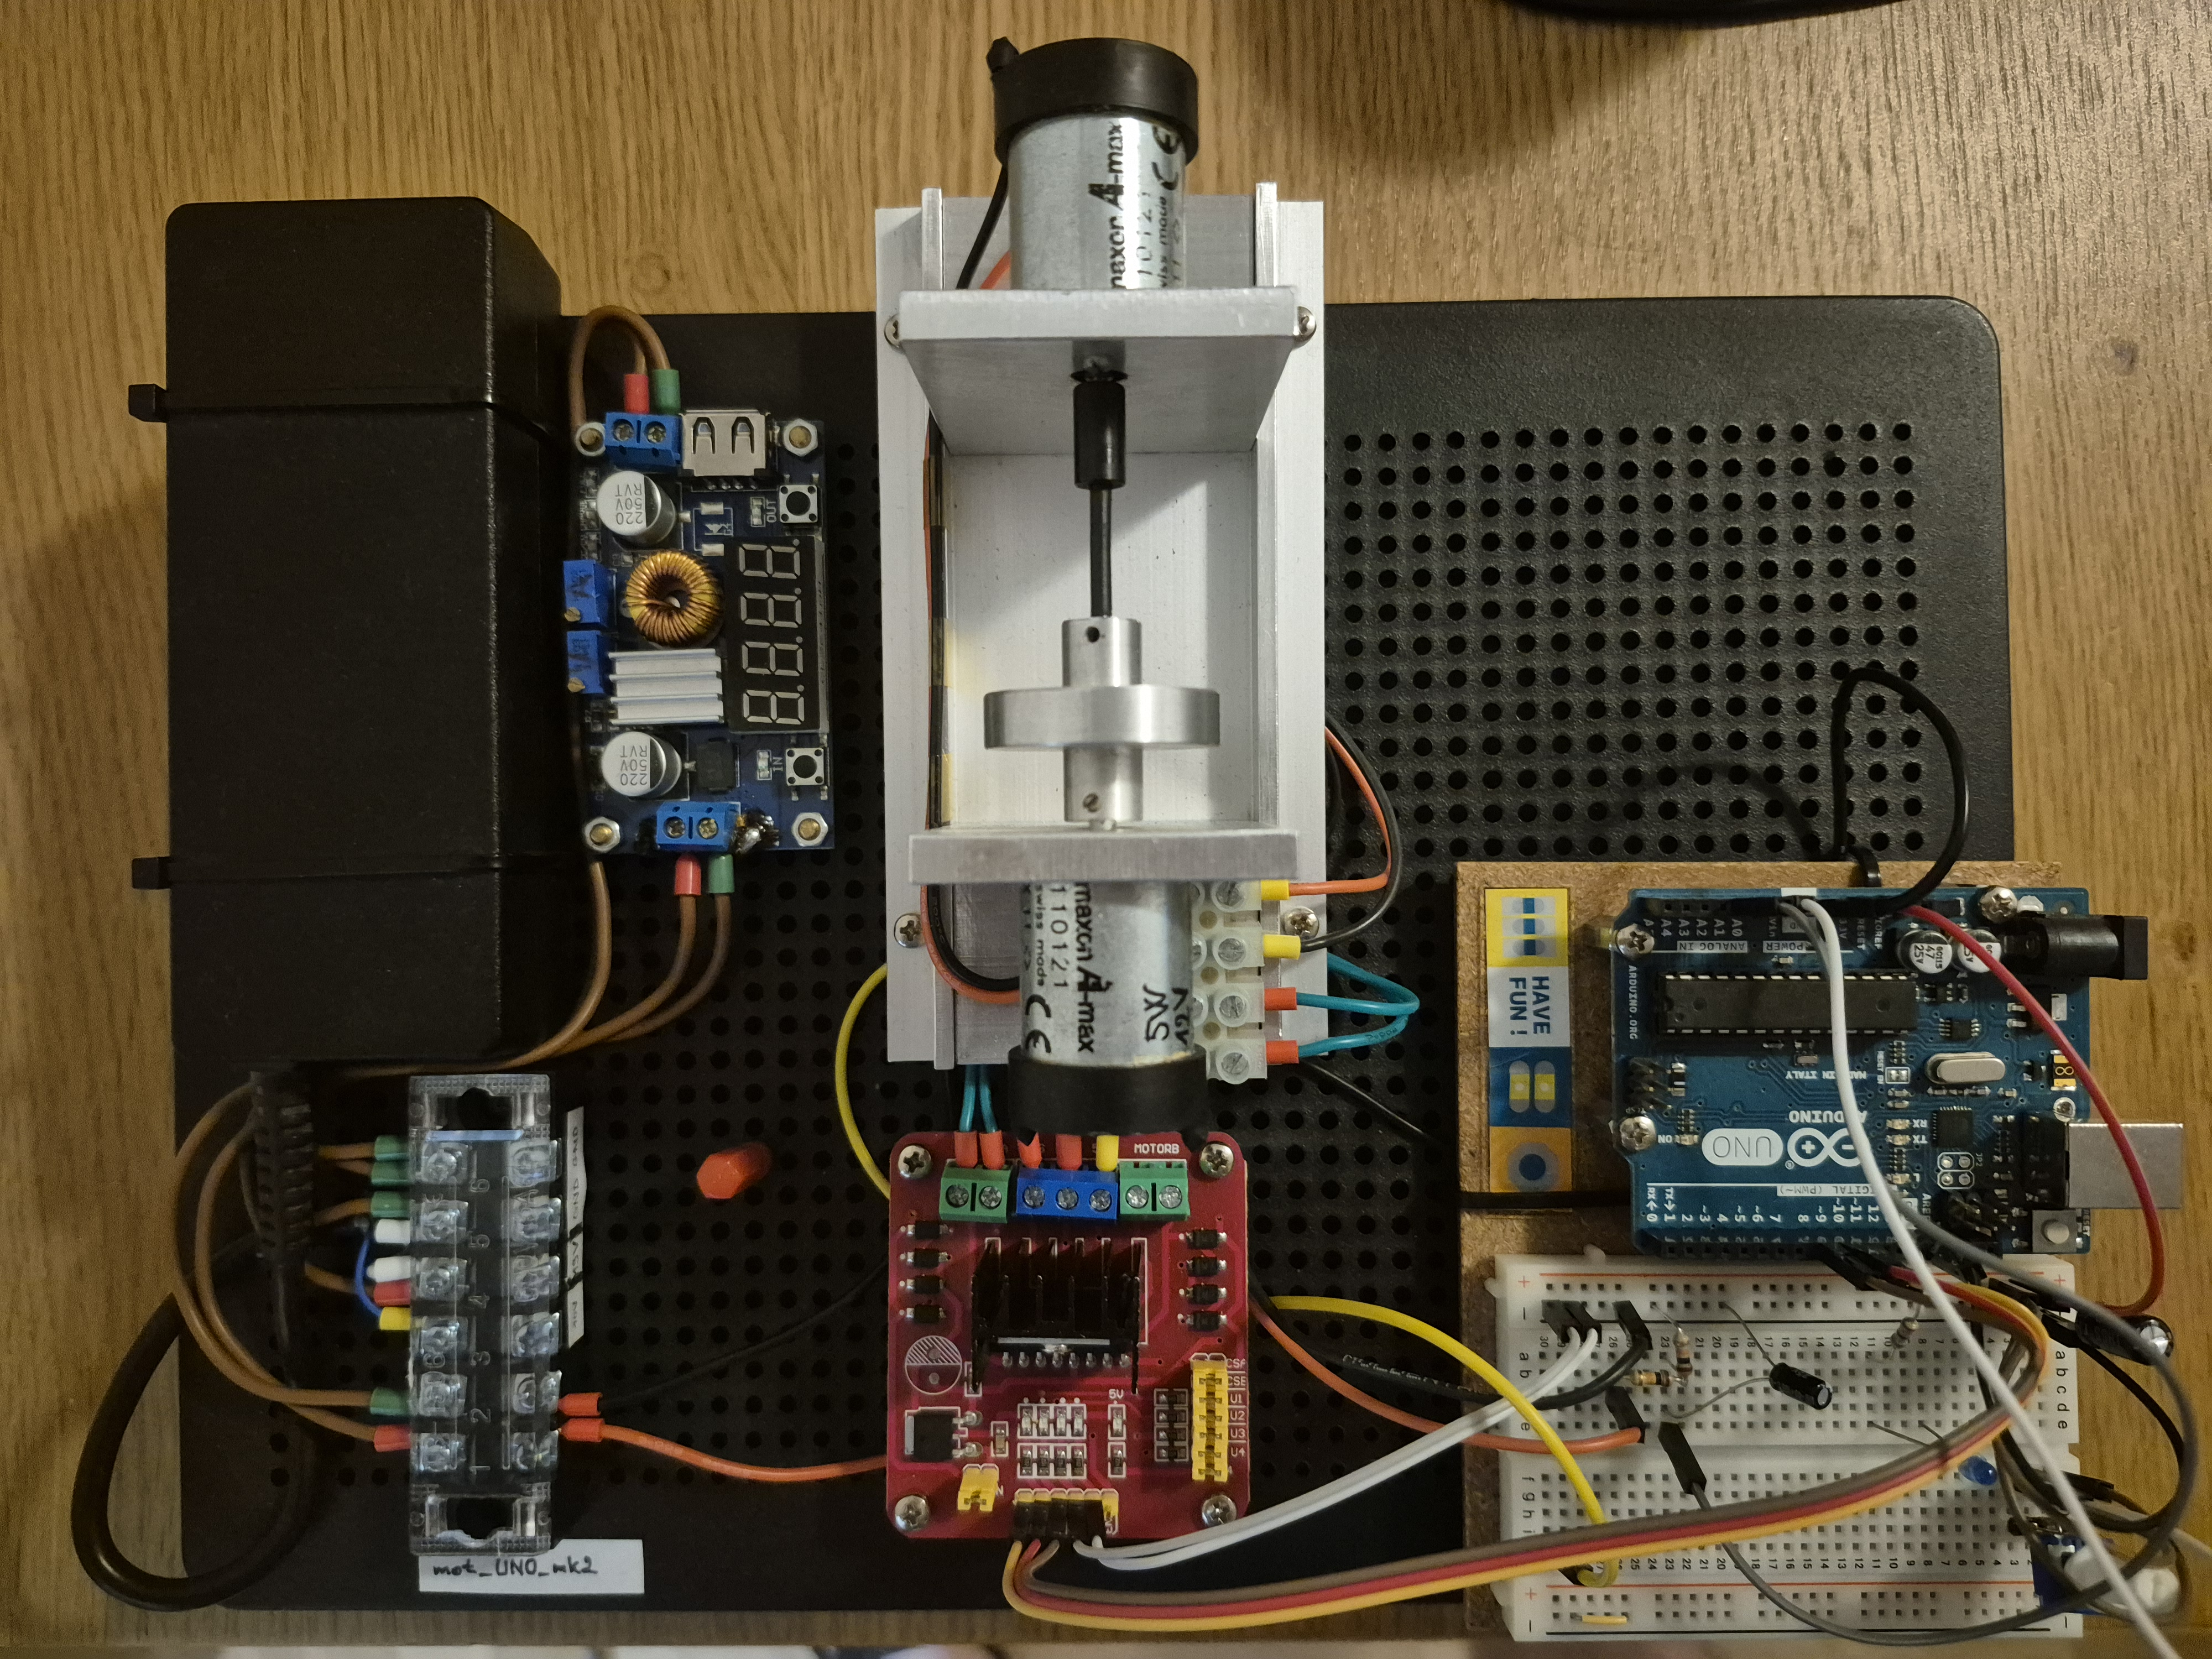
\includegraphics[width=1.2\textwidth,keepaspectratio]{motor-foto.jpg}
        }


        \figcaption{ 
            Fotografia.
        }
        \label{motor-foto}
    }%vbox

\end{center}







% -----------------------------------------------------------------------------

\end{document}

% -----------------------------------------------------------------------------